\documentclass[12pt]{article}

\usepackage{microtype}

\usepackage[T1]{fontenc}
\usepackage{mathpazo}
\usepackage{amsmath,amsthm}
\newtheorem{theorem}{Theorem}
\newtheorem{proposition}{Proposition}
\newtheorem{definition}{Definition}
\newtheorem{lemma}{Lemma}
\newtheorem{exercise}{Exercise}
\newtheorem{example}{Example}
\newtheorem{corollary}{Corollary}

\usepackage{algpseudocode}
\usepackage{listings}
\lstset{basicstyle=\ttfamily}

\usepackage{tcolorbox}
\newtcolorbox{examplebox}[1]{width=\textwidth,colback={lightgray},title={#1},colbacktitle={lightgray!50},coltitle={black}}
\newtcolorbox{algobox}[1]{width=\textwidth,colback={lightgray},title={#1},colbacktitle={lightgray!50},coltitle={black}}

\usepackage{tikz}
\usetikzlibrary{shapes,snakes,positioning,decorations.pathreplacing}

\usepackage{answers}
\Newassociation{sol}{Solution}{ans}
\Newassociation{hint}{Hint}{hints}



\usepackage{complexity}

\newcommand{\AND}{\lang{AND}}
\newcommand{\OR}{\lang{OR}}
\newcommand{\NOT}{\lang{NOT}}

\newcommand{\MATCHING}{\lang{MATCHING}}
\newcommand{\CLIQUE}{\lang{CLIQUE}}
\newcommand{\IS}{\lang{IS}}
\newcommand{\CVAL}{\lang{CVAL}}
\newcommand{\CSAT}{\lang{CSAT}}
\newcommand{\UNSAT}{\lang{UNSAT}}
\newcommand{\TAUT}{\lang{TAUT}}
\newcommand{\TQBF}{\lang{TQBF}}
\newcommand{\GNI}{\lang{GNI}}
\newcommand{\SharpSAT}{\lang{\#SAT}}
\newcommand{\REACH}{\lang{REACH}}
\newcommand{\PIT}{\lang{PIT}}

\newcommand{\lA}{\lang{A}}
\newcommand{\lB}{\lang{B}}
\newcommand{\lC}{\lang{C}}

\newcommand{\cC}{\class{C}}
\newcommand{\SharpP}{\class{\#P}}

\newcommand{\mM}{\class{M}}
\newcommand{\mU}{\class{U}}

\newcommand{\polym}{\leq_m^p}
\newcommand{\polyt}{\leq_T^p}


\title{Basic Complexity Theory}
\author{Balagopal Komarath}


\begin{document}

\maketitle

\section{Structural Complexity vs Low Level Complexity}

Structural complexity deals with high-level questions related to
computation: Are problems that are efficiently verifiable the same as
problems that are efficiently solvable ($\P$ vs $\NP$)? Low Level
complexity deals with the computational power/limitations of specific
computational models: Can the parity of arbitrary length bit strings
be computed by circuits with AND, OR, and NOT gates with constant
delay? In this book, we will deal with structural complexity. i.e.,
the questions we consider and the theorems we prove are concerned with
properties of the abstract notion of computation without being tied to
any particular computational model.

In \ref{languages}, we define the notion of decision problems and
languages associated with them. We also consider the issue of
encodings which specify the form in which a computational device
accepts input and produces output. The complexity of problems depend
upon the form in which the input is presented and the form of the
expected output. For example, consider the problem of adding two
natural numbers. If the inputs are in decimal notation, then one has
to use an algorithm like the usual digit-by-digit addition with carry
propagation to compute the sum. On the other hand, if the numbers are
presented in unary, then one can compute the sum by simply
concatenating the two numbers.

Even though we want to discuss the abstract notion of computation, it
is necessary to consider some concrete computational model to
formulate and prove statements. But, if we are using a concrete
computational model to prove our theorems, how can we ensure that
these statements hold for computation in general. In \ref{TM}, we
define a computational model -- The Turing Machine -- that is widely
believed to be equivalent (with respect to the questions we consider)
to any computational model realizable in the physical world. i.e., we
believe that the answers remain the same even if we replace Turing
Machines with any computational model.

In \ref{TimeSpace}, we define the time taken and space used by a
computation in a Turing Machine. We will also justify using order
notation to specify time and space complexity by showing that we can
arbitrarily improve the computation speed and space used by constant
factors. In \ref{Hierarchy}, we prove that giving TMs more time/space
strictly increases their power. The proof of this theorem is enabled
by showing that efficient interpreters exist.

In \ref{PvsNP}, we define the two most important classes of problems
and state the central question of complexity theory -- Are problems
that are efficiently verifiable the same as problems that are
efficiently solvable ($\P$ vs $\NP$)?

The $\P$ vs $\NP$ problem is about determining the absolute hardness
of problems. An endeavour which has been met with little
success. However, we show that we can prove relative hardness of
problems using algorithms\footnote{usually, algorithms are used to
  show that problems are easy} itself. In \ref{Reductions}, we define
these special algorithms, called reductions, that can be used to show
hardness of problems. This is followed by using reductions to show
that all complexity-related aspects of complexity classes are present
in certain problems called complete problems for the class in
question.

\section{Languages}

Decision Problems: Given a problem instance $x\in \{0, 1\}^*$, answer
yes or no. Examples of decision problems include ``Does the given
graph $G$ has a perfect matching?'' and ``Does the given graph $G$ has
a clique of size $k$ for the given number $k$?''. When talking about
computational problems, we have to fix an encoding of the input. In
the above examples, we typically assume that graphs are presented as
adjacency matrices or adjacency lists and numbers are encoded using
binary representation.

Languages: A language $L\subseteq \{0, 1\}^*$ corresponds to the
decision problem ``is $x\in L$?''. Also, every decision problem
naturally corresponds to the language containing all ``yes''
instances.

\begin{examplebox}{Languages}
\begin{itemize}                                            
  \item $\MATCHING = \{G : G \text{ has a perfect matching}\}$
  \item $\CLIQUE = \{(G, k) : G \text{ has a clique on $k$ vertices}\}$
\end{itemize}
\end{examplebox}

\section{Turing Machines}

Formal Definition. 

Turing machines can be thought of as special-purpose computers --
computers designed to run a specific algorithm. We will draw an
analogy to digital computers to claim that TMs represent computation
faithfully. The finite state machine stores the internal state
(Registers). The machine has a read-only input tape and constant
number (Say $k$) of work tapes (RAM) and a tape head for each tape
. The number $k$ can be thought of as the bus width, which is
bounded. The machine can read the symbol under the tape heads at each
step. Therefore, a TM can read exactly $k$ symbols from memory in one
step. At each step, the TM makes a decision based on the internal
state and contents under tape heads.  At each step, the TM can
overwrite cells under the tape heads (memory writes to a fixed number
of locations), change internal state (register writes) and move tape
heads one position left or right (sequential access to memory unlike
conventional processors). Since there are only a bounded number of
possibilities for the internal state and contents of $k$ tape cells
($|Q|.|\Sigma|^k$ to be exact), the transition table (control logic
inside the processor) is finite. This means that in a single step the
machine has access to and can modify/write to only finite piece of
information. This restriction is natural when considering physically
realized computational models. For example, each ASM instruction can
read from and write to only a fixed number of registers and a fixed
number of memory locations. When a person is performing computations
on a piece of paper, he/she only looks at two or three symbols on the
paper at a time and writes down at most one symbol at a time. The
fundamental elements of computation in a digital circuit, gates, have
fan-in and fan-out typically restricted to at most three. The
sequential access restriction to the work tapes is more unusual. This
means that TMs cannot represent certain algorithms -- such as binary
search -- faithfully. But, for the classes of problems we are going to
study, this restriction is irrelevant.

Extended Church-Turing Thesis: Any physically realizable computational
model can be simulated efficiently (with polynomial overhead) by some
TM. On the other hand, we also assume that any reasonable
computational model can simulate TMs efficiently. Together, these two
requirements ensure that our theorems about computation are indeed
about computation and not about specific computational models.

\section{Time and Space}

Definition of time and space complexity (worst-case) and associated
complexity classes.

The theorems below show that constants do not matter when analyzing
time and space complexity.

Linear speedup: Simulate $m$ steps of $\mM$ using 7 steps of a new
machine $\mM'$. Each cell in $\mM'$ holds $m$ symbols of a cell in
$\mM$ and in 4 steps $\mM'$ can scan and store all the symbols in the
current cell, the one to the left, and the one to the right in its
state machine (One move to the left, two moves to the right, and one
move to the left). In the next three steps, the machine $\mM'$ will
modify those 3 cells to reflect the operations performed by $\mM$ in
the next $m$ steps. Initially, compressing the input string requires
$n+1$ steps. Therefore, if $\mM$ takes $f(n)$ steps to complete, the
machine $\mM'$ takes $n+1+7f(n)/m$ steps to perform the same
computation. Assuming $f(n) \geq n$, we can achieve arbitrarily
speedup the computation by a constant factor. This proves that
analyzing constant factors in time complexity is useless.

Space compression: As in the above proof, each cell of worktapes hold
$m$ symbols from the original worktape alphabet. We do not re-encode
the input string into a new tape as this would make the space
complexity atleast linear. The machine $\mM'$ simulates a single step
of $\mM$ using a single step by rewriting the symbol on the current
work tape cells and the tape heads are moved left/right/stay
appropriately. The space taken is at most $\lceil f(n)/m \rceil$.

So the reason why constants do not matter is a direct consequence of
us not fixing the number of tapes and the alphabet size to specific
values. Therefore, these statements are not fundamental aspects of
computation but peculiarities of the TM.

Can 2-tape binary Turing machines be simulated with constant factor
overhead by such machines? Don't think so.

What happens if we define time and space in terms of information
content? The big questions do not change.

\section{Hierarchy Theorems}

Recall the diagonalization technique used to prove that there are no
bijections from natural numbers to the set of all functions on natural
numbers.

Encoding Turing Machines

Specify some binary encoding that is prefix-free.

\subsection{Universal Turing Machines}

In this section, we will prove that efficient interpreters exist. An
observation that would appear trivial in this day and age but needed a
proof in the 60's. A Turing machine is an encoding of an algorithm. A
Universal Turing machine takes a description of a Turing machine
(which is a description of an algorithm) and an input to that
algorithm as inputs and computes the result of executing the algorithm
on that input. i.e., a Universal Turing machine is simply an
interpreter for Turing machines. We are also interested in the
performance of the resulting interpreter. Specifically, we prove

\begin{theorem}
  There exists a Turing Machine $\mU$ given $(\mM, x)$ as input
  computes $\mM(x)$ in at most $|\mM|^2.t^2$ steps using at most
  $|\mM|.s$ cells where $\mM$ takes $t$ steps and uses $s$ cells on
  input $x$.
\end{theorem}

Enumerating Time and Space Bounded Turing Machines

Time and space constructibility are required here.

Time Hierarchy:

Mention Hennie-Stearns simulation that gives better time hierarchy
theorems.

The $\log(t)$ overhead during simulation is not a fundamental aspect
of computation. If we fix our computational model to a random access
machine and consider only languages over the binary alphabet, then a
constant factor overhead simulation is possible (A.G. Ivanov
1982). This shows that the precise statement of the time hierachy
theorem depends on the computational model being considered. But, the
time hierarchy theorem holds in some form for any reasonable
computational model as seen in Exercise~\ref{}.

Space Hierarchy:

\section{$\P$ vs $\NP$}

The precise statements of theorems in previous sections such as
speedup theorem, compression theorem, and hierarchy theorems were
closely tied to the specific model (TM) we used to define
computation. The statements we make from now on are applicable to any
reasonable computational model and are therefore considered
fundamental aspects of computation (as opposed to aspects of specific
computational models).

\subsection{Efficiently Solvable Problems}

$\P$ is the class of languages decidable in polynomial time and is
generally regarded as encompassing all problems that can be solved
efficiently in practice.

\begin{definition}
  $\P = \bigcup_{k\geq 1} \DTIME(n^k)$
\end{definition}

Class $\P$ is invariant to the model by extended Church-Turing thesis.

\begin{examplebox}{Examples for languages in \P}
 $\CVAL = \{(C, x) : \text{The Boolean circuit $C$ on input $x$ evaluates to 1}\}$
\end{examplebox}

In the above example, we assume that the Boolean circuit consists of
2-input AND gates, 2-input OR gates, 1-input NOT gates, input gates
labelled by one of the $n$ input variables, and constant gates of
value $0$ or $1$. A possible encoding of the circuit is given
below. We assume that gate $0$ is the output gate.

\begin{examplebox}{An encoding for circuits}
  \begin{lstlisting}[language=c]
struct circuit
{
  int m; /* Number of gates */
  int n; /* Number of input variables */
  struct gate_description
  {
    int gate_number;
    enum { AND, OR, NOT, IN, CONST } type;
    union
    {
      /* For AND, OR. 0 <= ingate1, ingate2 < m */
      struct { int ingate1; int ingate2; };
      /* For NOT. 0 <= ingate < m */
      int ingate;
      /* For IN. 0 <= input < n */
      int input;
      /* For CONST. value == 0 || value == 1 */
      int value;
    } gate_in;
  } gates[m];
};
\end{lstlisting}
\end{examplebox}

\begin{exercise}
  Show that $\P\subseteq \DTIME(n^k)$ for some constant $k$ is
  impossible in any reasonable computational model.
\end{exercise}

\begin{exercise}
  Show that for any reasonable computational model
  $\DTIME(f(n)) \subset \DTIME(f'(n))$ for any $f(n)$ where $f'(n)$ is
  only polynomially larger than $f(n)$.
\end{exercise}

\begin{exercise}
  Show that the class $\P$ is invariant under all reasonable
  computational models.
\end{exercise}

\subsection{Efficiently Verifiable Problems}

$\NP$ is the class of languages where for all strings in the language
there is atleast one certificate of length polynomial in the length of
the string that can be used along with the input to verify in
polynomial time that the input indeed is a member of the language. All
languages in $\P$ are in $\NP$. Examples for languages in $\NP$ not
known to be in $\P$ include \CLIQUE, \CSAT, and \IS.

\begin{examplebox}{Examples for languages in \NP}
  \begin{itemize}
  \item $\CSAT = \{C : \text{The Boolean circuit $C$ has a satisfying assignment}\}$
  \item $\IS = \{(G, k) : G \text{ has an independent-set on $k$ vertices}\}$
  \end{itemize}
\end{examplebox}

\begin{exercise}
  Show that the class $\NP$ is invariant under all reasonable
  computational models.
\end{exercise}

\section{Reductions}

Algorithms are usually used to solve problems. Sometimes we use
algorithms to connect two problems and prove that one is easier/harder
than the other. These algorithms are called \emph{reductions}.

A reduction from A to B for the complexity class $\P$ should show that
the statement $\lB\in \P \implies \lA\in \P$ is true. i.e., if $\lB$
is easy to solve, then $\lA$ is easy to solve as well.  Similarly, a
reduction from $\lA$ to $\lB$ for the complexity class $\NP$ should
show that the statement $\lB\in \NP \implies \lA\in \NP$ is
true. i.e., if $\lB$ is easy to verify, then $\lA$ is easy to verify
as well.

In general, given a complexity class $\cC$, a reduction is an
algorithm that shows that if $\lB\in \cC$, then $\lA\in \cC$. The
existence of such an algorithm is denoted by $\lA\leq \lB$.

Any notion of reduction should satisfy the following properties.

\begin{enumerate}
\item Reflexivity: For all languages $\lA$, we have $\lA\leq \lA$.
\item Transitivity: If $\lA\leq \lB$ and $\lB\leq \lC$, then $\lA\leq \lC$.
\end{enumerate}

We show a reduction from $\CLIQUE$ to $\IS$ below. Note that the
adjacency matrix of $\overline{G}$ can be computed from the adjacency
matrix of $G$ in linear time by simply flipping all the
bits. Therefore, if there is an algorithm for $\IS$ that runs in
$O(n^c)$ time for some constant $c$, then the following algorithm for
$\CLIQUE$ also runs in $O(n^c)$ time.

\begin{algobox}{Reduction from \CLIQUE\ to \IS\ for \P}
\begin{algorithmic}
    \Function{CLIQUE}{$G$, $k$}
        \State Compute $\overline{G}$, the complement of $G$.
	\State \Return \Call{IS}{$\overline{G}$, $k$}
    \EndFunction
\end{algorithmic}
\end{algobox}

In general, any algorithm for \lA\ that uses an algorithm for \lB\ as
a subroutine and runs in polynomial time assuming that the algorithm
for \lB\ runs in polynomial time is a reduction from \lA\ to \lB\ for
the class $\P$. Such reductions are called poly-time Turing reductions
and the existence of such a reduction is denoted by $\lA\leq_T^p \lB$.

The following algorithm shows that any language $\lA$ is reducible to
its complement using poly-time Turing reductions.

\begin{algobox}{Reduction from $\lA$ to $\lang{\overline{A}}$ for \P}
\begin{algorithmic}
    \Function{A}{$x$}
        \State \Return $\neg\Call{$\overline{A}$}{$x$}$
    \EndFunction
\end{algorithmic}
\end{algobox}

Does the reduction from \CLIQUE\ to \IS\ work for $\NP$? No. Because,
it does not show the existence of a poly-time verifier for
\CLIQUE\ given one for \IS. However, it can be easily modified to work
for $\NP$.

\begin{algobox}{Reduction from $\CLIQUE$ to $\IS$ for \NP}
\begin{algorithmic}
    \Function{CLIQUE-VERIFY}{$G$, $k$, $C$}
        \State Compute $\overline{G}$, the complement of $G$.
	\State \Return \Call{IS-VERIFY}{$\overline{G}$, $k$, $C$}
    \EndFunction
\end{algorithmic}
\end{algobox}

Now, if there is a poly-time verification algorithm for $\IS$, the
algorithm $\Call{CLIQUE-VERIFY}{}$ is a poly-time verification
algorithm for $\CLIQUE$.

The above transformation does not work for the reduction from \lang{A}
to $\lang{\overline{A}}$. In general, the transformation works for
reductions that have the following structure.

\begin{algobox}{A generic reduction from $\lA$ to $\lB$ for $\P$}
\begin{algorithmic}
    \Function{A}{$x$}
        \State $x' \gets \Call{f}{x}$
	\State \Return \Call{B}{$x'$}
    \EndFunction
\end{algorithmic}
where \Call{f}{} is a poly-time algorithm.
\end{algobox}

Such reductions are called poly-time many-one reductions and the
existence of such a reduction from $\lA$ to $\lB$ is denoted by
$\lA\leq_m^p \lB$. Such reductions work for both $\P$ and $\NP$.

\begin{proposition}
  \begin{enumerate}
  \item $\lA\leq_m^p \lB$ and $\lB\in \P$ implies $\lA\in \P$
  \item $\lA\leq_m^p \lB$ and $\lB\in \NP$ implies $\lA\in \NP$
  \end{enumerate}
\end{proposition}
\begin{proof}
  \begin{enumerate}
  \item $\lA\polym \lB$ implies $\lA\polyt \lB$.
    
  \item Given a poly-time many-one reduction from $\lA$ to $\lB$, we
    can write a poly-time verifier for $\lA$ given one for $\lB$ as
    follows.
    
    \begin{algobox}{Reduction from $\lA$ to $\lB$ for $\NP$}
      \begin{algorithmic}
        \Function{A-VERIFY}{$x$, $y$}
        \State $x' \gets \Call{f}{x}$
	\State \Return \Call{B-VERIFY}{$x'$, $y$}
        \EndFunction
      \end{algorithmic}
      where \Call{f}{} is a poly-time algorithm.
    \end{algobox}
  \end{enumerate}
\end{proof}

Note that a poly-time many-one reduction is completely described by
the function \Call{f}{} that transforms a problem instance for $\lA$
into a problem instance for $\lB$. Therefore, a poly-time many-one
reduction can be thought of as encoding instances of one language as
instances of another language.

\begin{definition}
  $\lA \polym \lB$ if and only if there exists a poly-time algorithm
  \Call{f}{} such that for all $x\in \{0, 1\}^*$, we have $x\in\lA
  \iff \Call{f}{x}\in\lB$.
\end{definition}


\begin{exercise}
  Are the following notions of reduction valid for $\NP$?
  
  \begin{algobox}{A reduction from $\lA$ to $\lB$ for $\NP$}
    \begin{algorithmic}
      \Function{A}{$x$}
      \State $x' \gets \Call{f}{x}$
      \State $x'' \gets \Call{g}{x}$
      \State \Return \Call{B}{$x'$} $\vee$ \Call{B}{$x''$}
      \EndFunction
    \end{algorithmic}
    where \Call{f}{} and \Call{g}{} are poly-time algorithms.
  \end{algobox}

  \begin{algobox}{A reduction from $\lA$ to $\lB$ for $\NP$}
    \begin{algorithmic}
      \Function{A}{$x$}
      \State $x' \gets \Call{f}{x}$
      \State $x'' \gets \Call{g}{x}$
      \State \Return \Call{B}{$x'$} $\wedge$ \Call{B}{$x''$}
      \EndFunction
    \end{algorithmic}
    where \Call{f}{} and \Call{g}{} are poly-time algorithms.
  \end{algobox}
  
\end{exercise}

\section{Complete Problems}
The class $\NP$ contains many problems such as $\CSAT$ and optimizing
integer linear programs that are not known to be in $\P$ but are
practically applicable. Is it possible that even though $\P\neq \NP$,
we could find poly-time algorithms for these practically relevant
problems. Cook showed that this is impossible by proving that the
question whether $\CSAT$ has a poly-time algorithm and the question
whether $\P = \NP$ is the same problem.

\begin{theorem}
  $\CSAT\in\P \iff \P=\NP$
\end{theorem}

One direction of this theorem is easy. If $\CSAT\not\in\P$, then
$\P\neq\NP$ because $\CSAT$ is a problem in $\NP$ that is not in
$\P$. The other direction is proved by showing that $\CSAT$ is harder
than any problem in $\NP$.

\begin{lemma}
  If $\lA\in\NP$, then $\lA\polym\CSAT$.
\end{lemma}

Even though the proof of this lemma is technically involved, the idea
behind the proof is very intuitive. Think of the poly-time verifier as
an algorithm running on a digital computer. The verifier takes the
pair $(x, y)$ as input where $x$ is the instance and $y$ is the
proof. Now, given an $x$ as instance to $\lA$, we can fix this part of
the input to the verifier and think of the $y$ part as $\poly(n)$
Boolean variables. The circuitry of the computer is made up of $\AND$,
$\OR$, and $\NOT$ gates. Therefore, we can view the computation of the
verifier as a circuit taking $y$ as input and producing the result of
the verifier on input $(x, y)$ as output. Let $C$ be this
circuit. Then, deciding whether there exists a $y$ such that $(x, y)$
is accepted by the verifier is the same as deciding whether there
exists a $y$ that makes $C$ output $y$.

However, there is a little problem. The circuitry inside a computer is
not combinational. However, the instances to the $\CSAT$ problem are
combinational circuits. The are directed cycles in the circuit arise
from the need for updating registers and memory. For example, A part
of the circuit reads registers, computes new values, and writes new
values to registers leading to a loop.The key observation made by Cook
was that we can ``unroll'' these circuits by constructing copies of
elements in the original circuit to create an equivalent combinational
circuit. Take the previous example of register updation. We can remove
this loop by making two sets of register files. The circuit will read
from the first register file and write to the second register file. If
the machine runs for $m$ steps, then we have to make $m$ copies of the
register file and the update circuitry to avoid loops. Similarly, we
can make $m$ copies of all the memory cells and the associated update
circuitry used by the verifier to avoid loops. Since the total number
of instructions taken is at most $p(n)$, at most $p(n)$ copies of the
original circuit is sufficient to avoid all loops. Therefore, the
circuit $C$ has size atmost $kp^2(n)$ for some constant $k$. The proof
of Lemma~\ref{} is essentially this idea implemented in the world of
Turing machines.

\section{Space, \L, \NL, and Savitch's Theorem}

The complexity class $\L$ is the set of all problems solvable using at
most $c\log(n)$ work tape cells for some constant $c$. It is
considered as the class of all problems solvable efficiently where the
complexity measure is space.

The analogue of the class $\NP$ in this setting, called class $\NL$ is
the class of all problems efficiently verifiable in terms of
space. Formally, we can define the class in terms of read-once proofs
verifiable using logspace.

logspace reductions and $\SAT$ is complete for $\NP$ under logspace.

The positions of head tapes are computable in logspace. The logspace
reducer can output the circuit layer by layer. Each cell is updated
using a circuit that takes only constant many bits as input.

\begin{exercise}
  Show that if we allow two-way access to the proof and restrict the
  verifier to logspace, then we get the class $\NP$.
\end{exercise}

\begin{exercise}
  Consider a read-once proof verifier that uses $c\log(n)$ space.
  Show that if the verifier can be made to accept a read-once proof of
  length more than $2^{c\log(n)}$, then there is a read-once proof of
  length at most $2^{c\log(n)}$ that is accepted by the verifier.
\end{exercise}

completeness of \REACH.

\begin{algobox}{Savitch's Algorithm}
  \begin{algorithmic}
    \Function{REACH-N}{$s$, $t$, $n$}
    \ForAll{$v\in V$}
    \If{\Call{REACH-N}{$s$, $v$, $n/2$} $\wedge$ \Call{REACH-N}{$v$, $t$, $n/2$}}
    \State \Return true
    \EndIf
    \EndFor
    \State \Return false
    \EndFunction
  \end{algorithmic}
\end{algobox}

The depth of the recursion is $O(\log(n))$ and at each level of the
recursion we only have to keep track of three vertices $s$, $t$, and
$v$ which takes up $O(\log(n))$ space.

\section{Co-classes and Inductive Counting}

$\co\NP = \{L : \overline{L}\in\NP\}$ and $\UNSAT$ and $\TAUT$ as
complete problems.

$\co\NL$ as the analogue.

\begin{exercise}
  Show that if $\NP\neq \co\NP$, then $\P\neq \NP$.
\end{exercise}

Define $r_i$ as the number of vertices reachable from $s$ in at most
$i$ steps from $s$. In particular $r_0 = 1$ and $r_{n-1}$ is the
number of vertices reachable from $s$.

Given $r = r_{n-1}$, it is easy to give a short read-once proof to
prove that $t$ is not reachable from $s$. Let $u_1 < \dotsm u_r$ be
the vertices reachable from $s$. Then the read-once proof is the
concatenation of $s$-$u_i$ paths for each $i$ from $1$ to $r$. The
verifier can verify this proof in logspace in read-once fashion.

But how do we get the value of $r_{n-1}$? We ask the prover to provide
it as a read-once proof. Assuming that we know $r_i$, we can construct
a read-once proof for $r_{i+1}$ as follows: The proof has a record for
each vertex $v$ in the graph in increasing order of $v$. If $v$ is
reachable from $s$ in at most $i+1$ steps, then give a path with at
most $i+1$ edges as proof. Otherwise, for each neighbour $u$ of $v$,
give a read-once proof of the fact that $u$ is not reachable from $s$
in at most $i$ steps. This is easy when $r_i$ is known as described in
the previous paragraph.

The structure of the read-once proof expected is given below.

\begin{examplebox}{Read-once proof for $\overline{\REACH}$}
proof of $r_1$. proof of $r_2$ given $r_1$ $\dotsc$ proof of $r_{n-1}$
given $r_{n-2}$. proof of $t$ not reachable from $s$ given $r_{n-1}$
\end{examplebox}

\section{The Polynomial Hierarchy}

The language $\TAUT$ is complete for $\co\NP$. Indeed, this problem
can be thought of as deciding whether $\forall x \phi(x)$ is true for
a given propositional formula $\phi$. In this way, the language $\SAT$
can be thought of as deciding whether $\exists x \phi(x)$ is true for
a given propositional formula $\phi$. What is the set of all languages
reducible to the problem of deciding whether
$\exists x \forall y \phi(x, y)$ is true for a given propositional
formula $\phi$? Observe that this set contains both $\NP$ and
$\co\NP$.

Oracle machines. $\mM^L$ is a TM that has access to an oracle that
decides $L$. Access to $\SAT$ is equivalent to access to any language
in $\NP$. Therefore, $\mM^\SAT$ is also written as $\mM^\NP$. The
class $\NP^\NP$ is the class of all languages verifiable in poly-time
by machines that have oracle access to $\SAT$. Note that if
$\P = \NP$, then $\NP^\NP = \P$.

Alternating Turing machines. A TM that can guess bits during
computation. Two types of guesses are allowed -- Existential and
Universal. Each guess causes the computation to diverge into $2$
independent threads with the value of the guessed bit set to $0$ and
$1$. For an input $x$, the computation of an ATM $M(x)$ can be
expressed as a rooted tree where each internal node is labelled
$\exists$ -- corresponding to existential guesses -- or $\forall$ --
corresponding to universal guesses. The leaves of the tree are
labelled accept or reject depending on whether the machine accepts or
rejects on the guessed bits leading to that leaf. An intermediate node
labelled $\exists$ is marked accept if at least one of its children is
marked accept and an intermediate node labelled $\forall$ is marked
accept if all of its children are marked accept. If there are at most
$k-1$ alternations in any path from root to leaf, then the machine is
$k$-alternating.  The time taken by the machine is the maximum of the
time taken by any of the threads. $\NP$ can be decided by
$1$-alternating ATMs with only existential guesses. $\co\NP$ with
$1$-alternating universal guesses. $2$-alternating with $\exists$
followed by $\forall$ called a $\exists\,\forall \class{ATM}$ can
decide any language in the above set. The language is complete for
this class by Cook's reduction.

Every $2$-alternating ATM with $\exists$ followed by $\forall$ can be
converted into a canonical form where the machine guesses $t(|x|)$
bits existentially, followed by universally guessing $t(|x|)$ bits,
followed by deterministic computation.

\begin{algobox}{Canonical $\exists\, \forall \class{ATM}$}
  \begin{algorithmic}
    \Function{M'}{x}
    \State Existentially guess $t(|x|)$ bits and write them to tape.
    \State Universally guess $t(|x|)$ bits and write them to tape.
    \State Simulate \Call{M}{x}. When \Call{M}{} makes an
    existential (universal) guess, use the next bit from the
    initially guessed existential (universal) bits.
    \EndFunction
  \end{algorithmic}
\end{algobox}

$\NP^\NP = \Sigma_2$

\begin{algobox}{$\exists\,\forall$ ATM for $\NP^\NP$}
  \begin{algorithmic}
    \Function{M'}{x}
    \State Existentially guess the certificate and the answers to queries of the $\SAT$ oracle.
    \State Universally guess the assignments for each formula not in $\SAT$ from the previous guess.
    \State Simulate \Call{M}{x}. When \Call{M}{} makes a query, use the guessed answer.
    If the guessed answer is $0$ and  the assignment guessed in second step satisfies the formula, reject.
    Accept if \Call{M}{} accepts.
    \EndFunction
  \end{algorithmic}
\end{algobox}

\begin{algobox}{$\NP^\NP$ verifier for $\exists x \forall y \phi(x, y)$}
  \begin{algorithmic}
    \Function{Verify}{$\phi$, $a$}
    \State Substitute $a$ for $x$ in $\phi$. The resulting formula $\phi'$ is on just the $y$ variables.
    \State Query the $\SAT$ oracle using $\neg\phi'$. If the result is $1$, reject, else accept.
    \EndFunction
  \end{algorithmic}
\end{algobox}

$\co\NP^\NP = \Pi_2$ is the class of languages decided by $\forall\,\exists\class{ATM}$.

Prove that $\Pi_i = \{L : \overline{L} \in \Sigma_i \}$

Inductively, we define $\co\NP^{\Sigma_i} = \Pi_{i+1}$ and
$\NP^{\Sigma_i} = \Sigma_{i+1}$. The equivalance between ATM, oracle
model, and problems reducible to formulas hold in general as well.

$\AP$ is the class of languages decided by poly-time ATMs. This class
is the same as $\PSPACE$.

\begin{algobox}{$\AP\subseteq\PSPACE$}
  \begin{algorithmic}
    \Function{M'}{$x$, $C$}
    \State Simulate \Call{M}{x} from configuration $C$.
    \State When \Call{M}{} makes a guess, let $C_0$ and $C_1$
    be the next configurations corresponding to guesses $0$ and $1$.
    \If{guess is $\exists$}
    \State \Return \Call{M}{x, $C_0$} $\vee$ \Call{M}{x, $C_1$}
    \EndIf
    \If{guess is $\forall$}
    \State \Return \Call{M}{x, $C_0$} $\wedge$ \Call{M}{x, $C_1$}
    \EndIf
    \EndFunction
  \end{algorithmic}
\end{algobox}

The machine \Call{M'}{x, C} simulates the computation of \Call{M}{x}
from configuration $C$. The algorithm \Call{M'} is invoked with
arguments $x$ and the initial configuration of \Call{M}{}.

The recursion depth is bounded by the time taken by the ATM. The
configurations of the ATM can be stored in polynomial
space. Therefore, the above algorithm uses only polynomial space.

\begin{algobox}{$\PSPACE\subseteq\AP$}
  \begin{algorithmic}
    \Function{M'}{$x$}
    \State $C_0\gets$ initial configuration of \Call{M}{x}.
    \State $C_1\gets$ accepting configuration of \Call{M}{x}.
    \State Existentially guess a configuration $C_m$ of \Call{M}{x}.
    \For{$i\gets 1 \text{ to } p(n)-1$}
    \State Universally guess a bit $b$.
    \State Existentially guess a configuration $C$ of \Call{M}{x}.
    \State $C_{1-b}\gets C_m$
    \State $C_m\gets C$
    \EndFor
    \State \Return true iff $C_0 = C_1$ or $C_0 \rightarrow C_1$ or  $C_0 \rightarrow C_m \rightarrow C_1$.
    \EndFunction
  \end{algorithmic}
\end{algobox}

Let \Call{M}{} take at most $p(n)$ space, where $n = |x|$. Let $(C_0,
\dotsc, C_{2^{p(n)}})$ be the sequence of configurations in the
computation \Call{M}{x} where $C_{2^{p(n)}}$ is the accepting
configuration. The machine $\Call{M'}{}$ recursively divides the
configuration sequence into equal sized halves by existentially
guessing the middle configuration $C_m$ and then uses universal
quantifier to check whether $C_m$ is reachable from $C_0$ and
$C_{2^{p(n)}}$ is reachable from $C_m$ in half the number of original
steps. This is simply an implementation of Savitch's algorithm in an
ATM.

We show that there is a proof tree for \Call{M'}{x}.  Let $r =
2^{p(n)}$. When $r = 2$, we simply guess $C_1$ and check
$C_0\rightarrow C_1\rightarrow C_2$. Assume that $r > 2$. For the
first existential guess, we assign the middle configuration
$C_{r/2}$. This splits the configuration sequence into two equal sized
halves. The subsequent universal and existential guesses occur in
pairs. For the first universal guess $b$ in the loop, when $b = 0$, we
only check whether $C_{r/2}$ is reachable from $C_0$ in at most $r/2$
steps. For this, we assign to the corresponding existential guess the
middle coniguration $C_{r/4}$ of the sequence $(C_0, \dotsc,
C_{r/2})$. When $b = 1$, we simply check whether $C_{r}$ is reachable
from $C_{r/2}$ in $r/2$ steps. For this, we assign the middle
configuration of the sequence $(C_{r/2}, \dotsc ,C_{r})$, i.e.,
$C_{3r/4}$, to the corresponding existential guess. Both these are
accepting by induction.

Figure~\ref{} shows the accepting proof tree for the sequence $(C_0,
\dotsc, C_8)$.

\tikzstyle{level 2}=[sibling distance=4cm]
\tikzstyle{level 4}=[sibling distance=2cm]
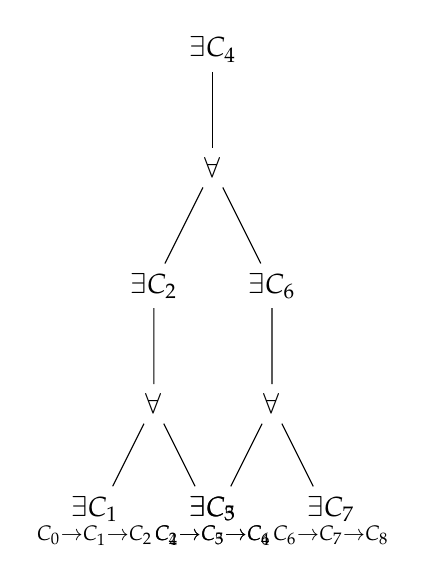
\begin{tikzpicture}
  \node {$\exists C_4$}
    child { node{$\forall$}
      child { node {$\exists C_2$}
        child { node {$\forall$}
          child { node {$\underset{C_0\rightarrow C_1\rightarrow C_2}{\exists C_1}$}}
          child { node {$\underset{C_2\rightarrow C_3\rightarrow C_4}{\exists C_3}$}}}}
      child { node {$\exists C_6$}
        child { node {$\forall$}
          child { node {$\underset{C_4\rightarrow C_5\rightarrow C_6}{\exists C_5}$}}
          child { node {$\underset{C_6\rightarrow C_7\rightarrow C_8}{\exists C_7}$}}}}};
\end{tikzpicture}

\begin{theorem}
  $\TQBF$ is complete for $\PSPACE$ under $\polym$ reductions.
\end{theorem}
\begin{proof}
  Membership is shown by a recursive algorithm that eliminates
  quantifiers one-by-one. For showing hardness, it is straightforward
  to convert the computation of the poly-time ATM to a QBF with $p(n)$
  alternations using Cook's reduction.
\end{proof}


Alternation by Chandra, Kozen, Stockmeyer.

\section{Counting}

\SharpP\ etc.

Toda's theorem.

\section{Interactive Proofs}

We show the containment $\IP \subseteq \PSPACE$ using a
straightforward algorithm.  Let $L \in \IP$ be the language of
interest. We show that it is possible to determine in \PSPACE\ whether
there exists a prover strategy that could make the verifier accept on
more than $3/4$ of the fraction of all random inputs. Since the input
$x$ is fixed, verifier's actions depends only on the random bits and
messages from the prover.

Let us say we have a function \Call{f}{$x, \gamma$} that implements
the optimal prover strategy.  Here $x$ is the common input and
$\gamma$ is the partial transcript of interaction. That is, $\gamma$
contains the sequence of messages exchanged between verifier and
prover until now.  The function \Call{f}{} returns the next message $m$ sent
by the (optimal) prover to receiver.

Given $f$ it is straightforward to compute whether $x \in L$. The
\PSPACE\ algorithm iterates over all possible choices of random string
and simulates the interaction between the optimal prover (implemented
by \Call{f}{}) and verifier and computes the fraction of random inputs
on which verifier accepts.

It remains to show $ \Call{f}{}$ can be implemented in polynomial
space. Let us look at all the information available to the prover to
determine the next message $m$ given $(x, \gamma)$. The prover has the
common input $x$ and the partial transcript $\gamma$. In addition the
prover ``knows'' verifier's (randomized) algorithm and hence will be
able to simulate the randomized algorithm. In other words, the only
information not available to the prover is the exact choice of random
bits available to the verifier in the current interaction.

The optimal prover will always choose a message $m$ that will maximize
the chance of acceptance.  Note that the verifier's acceptance depends
on both the prover's responses and the exact choice of random
bits. Even though the prover does not know the exact choice of random
bits, he can narrow it down to a subset of all possible choices. The
prover knows that the choice of random bits is such that the partial
transcript generated is $\gamma$. The next message chosen is the $m$
which maximizes the chance of verifier accepting $x$ where the
maximization is over all possible random strings $r$ consistent with
the partial transcript $\gamma$. Note that we may call the function
$f$ recursively to compute $\Call{f}{x, \gamma}$.  The algorithm in
full detail is given below. Here $r(n)$ denotes the total number of
random bits used , $p(n)$ denotes the length of the message, and $.$
denotes the concatenation operation.

\begin{algobox}{Simulating Prover in Polynomial Space}
  \begin{algorithmic}
    \Function{f}{$x, \gamma$}
    \ForAll{$m \in \Sigma^{p(n)}$}
    \ForAll{$r \in \Sigma^{r(n)}$ consistent with $(x, \gamma)$}
    \State Simulate $V$ using $r$ and partial transcript
    $\gamma . m$ calling \Call{f}{} to compute prover's messages.
    \EndFor
    \EndFor
    \State \Return $m$ for which $V$ accepted for the most random
    strings.
    \EndFunction
  \end{algorithmic}
\end{algobox}


The function \Call{f}{} is computable in polynomial space since the
depth of the recursion is polynomial. This is because all interactions
have only polynomial number of rounds and each call takes up
polynomial space.


\begin{algobox}{$\GNI\in \IP$}
  \begin{algorithmic}
    \State V: Choose a random permutation $\sigma\in S_n$ and $i\in\{0, 1\}$.
    \State V: Send $\sigma(G_i)$.
    \State P: Compute and send $i$.
  \end{algorithmic}
\end{algobox}

$\SharpSAT\in\IP$

Arithmetizing 3CNF formulas.

$C = x_i \vee \overline{x_j} \vee x_k \mapsto 1 - (1-X_i)X_j(1-X_k) = p_C$

$\phi \mapsto \prod_{C\in\phi} p_C = p_\phi(X_1,\dotsc,X_n)$

$p_\phi$ is a multilinear polynomial and has degree at most $3m$.

The prover has to provide $K$ and prove that
$K = \sum\limits_{b_1\in\{0,1\}}\dotso \sum\limits_{b_n\in\{0,1\}}
p_\phi(b_1,\dotsc,b_n)$

More generally, given a polynomial $g(X_1,\dotsc,X_n)$ of low-degree
$d$ prove that
$K = \sum\limits_{b_1\in\{0,1\}}\dotso \sum\limits_{b_n\in\{0,1\}}
g(b_1,\dotsc,b_n)$

Idea: A degree-$d$ univariate polynomial can have at most $d$ roots.

All evaluations are done modulo a prime $p\in(2^n, 2^{2n}]$.

Consider
$h(X_1) = \sum\limits_{b_2\in\{0,1\}}\dotso
\sum\limits_{b_n\in\{0,1\}} g(X_1,b_2,\dotsc,b_n)$

Prover sends a degree-$d$ univariate polynomial $s(X_1)$ claiming to
be $h(X_1)$.

Verifier checks $s(0) + s(1) = K$. Choose a random $a\in GF(p)$. Asks
the prover to prove
$s(a) = \sum\limits_{b_2\in\{0,1\}}\dotso \sum\limits_{b_n\in\{0,1\}}
g(a,b_2,\dotsc,b_n)$. $g(a,X_2,\dotsc,X_n)$ is a polynomial of
degree-$d$ on $n-1$ variables.

If the claimed count is right, the prover always sends the correct
polynomials and proof will be accepted by the verifier. If the claimed
count is wrong, then $s(X_1) \neq h(X_1)$ and therefore with
probability at least $(1-d/p)$, the prover has to prove a wrong
claim. By induction, the prover will fail with probability at least
${(1-d/p)}^{n-1}$ on the $(n-1)$ variable case. So in the $n$-variable
case, the verifier will reject with probability at least
${(1-d/p)}^{n}$. When $n = 1$, the verifier can compute the solution
and therefore will reject any wrong proof proving the base case.


$\TQBF\in\IP$

Consider the QBF
$\phi = \forall x_1 \exists x_2 \forall x_3 \exists x_4 \forall x_5
\bigl[ (x_1 \vee x_2 \vee x_3) \wedge (\overline{x_4} \vee
x_5)\bigr]$. Checking whether this is satisfiable is equivalant to
checking whether the following expression is non-zero.

\begin{equation*}
  \prod_{x_1\in\{0,1\}} \sum_{x_2\in\{0,1\}}  \prod_{x_3\in\{0,1\}} \sum_{x_4\in\{0,1\}}  \prod_{x_5\in\{0,1\}} P_\phi(x_1, x_2, x_3, x_4, x_5)
\end{equation*}

Therefore, we can try and run the protocol for \SharpSAT\ as
before. The problem is that each product gate could double the degree
of $x_1$ in $h(x_1)$ leading to an exponential (in $n$) degree
polynomial. This problem arises because there are $O(n)$ product gates
between the $x_1$ in $P_\phi$ and the product gate iterating over all
values of $x_1$ in the expression. Shamir observed that one can
convert any QBF $\phi$ to an equivalent formula $\phi'$ where the
number of universal quantifiers between any occurence of a variable
and the quantifier corresponding to the variable is at most $1$.

\begin{align*}
  \phi' = \forall x_1 \exists x_2 &\forall x_3 \exists x_1^1 \exists x_2^1\\
  &[(x_1^1 = x_1) \wedge (x_2^1 = x_2) \wedge\\
  &\exists x_4 \forall x_5 \bigl[ (x_1^1 \vee x_2^1 \vee x_3) \wedge (\overline{x_4} \vee x_5)\bigr]
\end{align*}

The equality $x_1^1 = x_1$ is the Boolean expression
$(x_1^1 \wedge x_1) \vee (\overline{x_1^1} \wedge \overline{x_1}) =
(x_1^1 \vee \overline{x_1}) \wedge (\overline{x_1^1} \vee x_1)$. Given
any satisfying assignment for $\phi$, we can set all copies of $x_i$
to the same value as $x_i$ in $\phi'$ and obtain a satisfying
assignment for $\phi'$. Given a satisfying assignment for $\phi'$, all
copies of $x_i$ will have the same value as $x_i$. Therefore, we can
obtain a satisfying assignment for $\phi$ from this assignment.

\begin{proposition}
$P(X)$ of degree-d has at most $d$ roots.
\end{proposition}
\begin{proof}
$P(X)$ has root $a$ if and only if $X-a$ is a factor. If $a$ is a
root, then $P(X) = Q(X)(X-a) + R$ and $R$ has to be a constant and
therefore $P(a) = R = 0$. If $X-a$ is a factor, then
$P(X) = Q(X)(X-a)$ and $P(a) = 0$.
\end{proof}

\section{The PCP Theorem and Inapproximability}

The model and statement of the PCP theorem.

Using PCP theorem to prove inapproximability.

\section{Low Depth Circuits}

The $\NC$ and $\AC$ classes.

$\AC0$ lower bounds using the polynomial method.

Uniform $\TC0$ lower bounds by Allender.

\section{Randomness}

Definitions of $\BPP$, $\RP$, $\co\RP$.

$\BPP\subseteq\Ppoly$

$\PIT$ as the poster problem for randomization.

Randomness vs Hardness

\section{Algorithms vs Lower Bounds}



\end{document}


